This chapter will go over methods and procedures used in the development of the DAQ system.
\section{Research and Design Phase}
\subsection{Research Phase}
During the research phase an exhaustive literature review was conducted.
When reviewing the designs for DAQ and GLV systems of other FSAE teams, the following points were looked for, in rough order of priority:
\begin{enumerate}
    \item Sensor and connector selection
    \item Methodology
    \item Overall system design
\end{enumerate}

\subsection{Electrical Design}
The DAQ package requires many components to be connected to different boards located throughout the car.
A spreadsheet was used to keep track of all components, their operating voltages, current draw, what microcontroller pin they would be accessible on, and which board they would be connected to.
\begin{figure}[H]
        \centering
        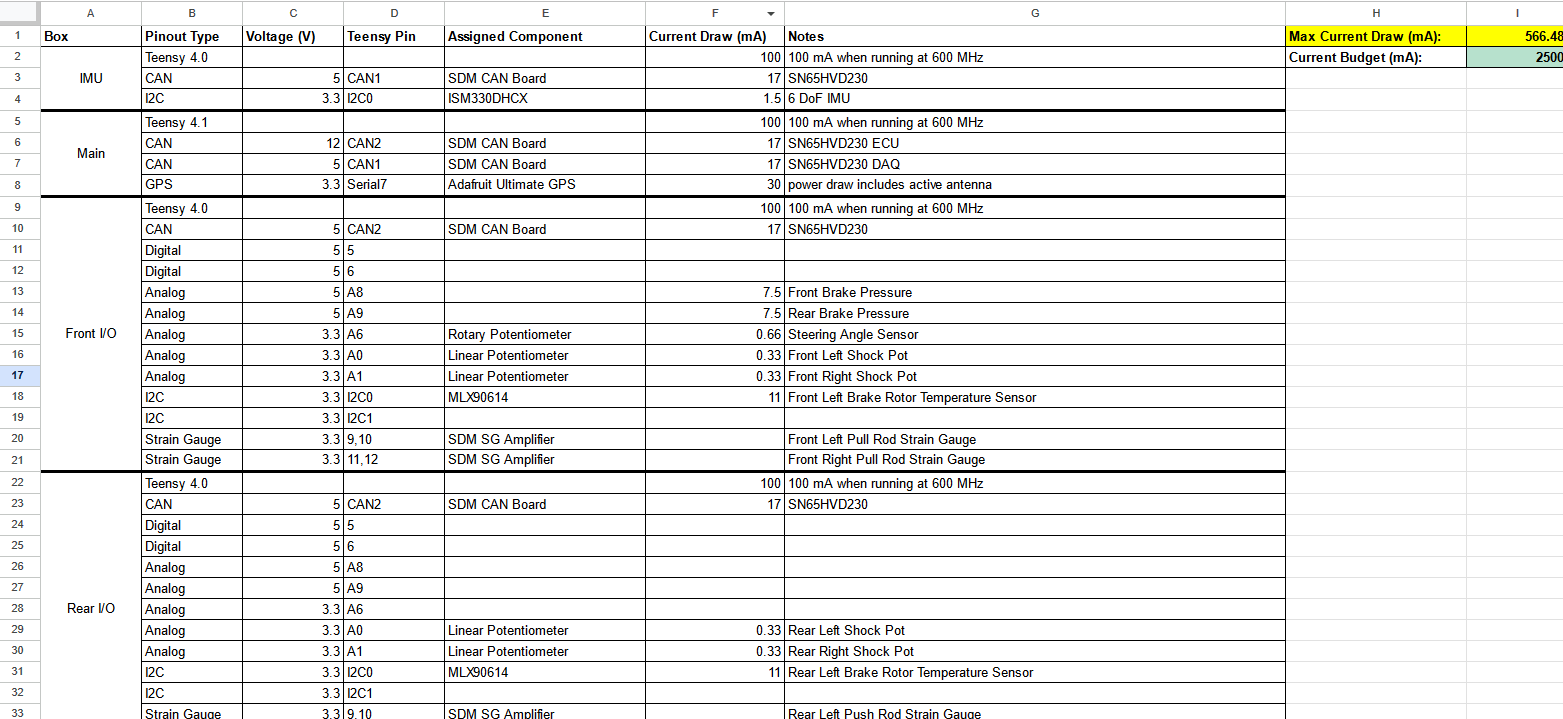
\includegraphics[width=7in]{images/electricalplanning.png}
        \caption{Component Planning Spreadsheet}
        \label{fig:ep}
\end{figure}


\subsection{Software Design}
PlatformIO, a VS Code extension, was used to develop software for the Teensy 4.1 and Teensy 4.0.
It is functionally equivalent to the Arduino IDE, while having the benefits of using a professional text editor such as VS Code.
Although not exclusive to PlatformIO, using this platform (i.e. Teensyduino) allows us to use Arduino functions and libraries for the Teensy boards, which greatly sped up software development.

\subsubsection{CAN Protocol Design}
The DAQ CAN bus will have to handle multiple channels of data of varying sizes.
Each CAN message contains 8 bytes of data, which is more than enough for one channel.
As such, some data channels, when encoded smartly, can be combined into a single message.
\vspace{1em}

The CAN protocol is described in a spreadsheet located on the team's Google Drive.
It includes information such as the CAN message ID, which component is sending the message, if it is signed or unsigned, the data channel being encoded, its units, and how to encode and decode the data.
Since the DAQ CAN bus is separate from the ECU's, message IDs that conflicted with the Haltech CAN protocol were not an issue.
\begin{figure}[H]
        \centering
        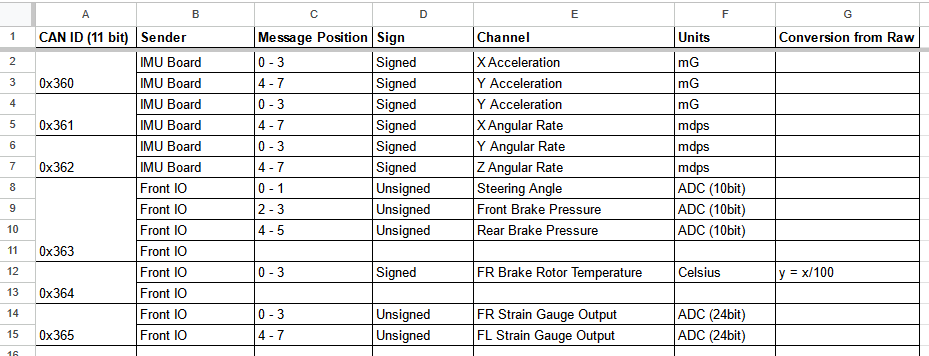
\includegraphics[width=6.5in]{images/canplanning.png}
        \caption{CAN Planning Spreadsheet}
        \label{fig:cpslol}
\end{figure}
\subsection{Hardware Design}
To simplify hardware designs and part orders, only M3 and 8-32 screws are used, unless a different size was required.


\section{Manufacturing Phase}
All printed circuit board (PCB) designs were created using KiCad and sent to JLCPCB for manufacturing.
Unless otherwise mentioned, any SMT assembly required were also done by JLCPCB.
Enclosures and sensor mounts were created using SOLIDWORKS and were either sent to AEI Industries for laser cutting with 6061 aluminum or 3D printed at ASU using PETG and PLA.

\subsection{Wiring and Pinout Documentation}
Three spreadsheets were maintained for wiring manufacturing:
\begin{itemize}
    \item Wire color conventions
    \item Wire length and assembly status
    \item Pinout documentation
\end{itemize}
The color convention spreadsheet showed all possible wire colors for each type of connection.
\begin{figure}[H]
        \centering
        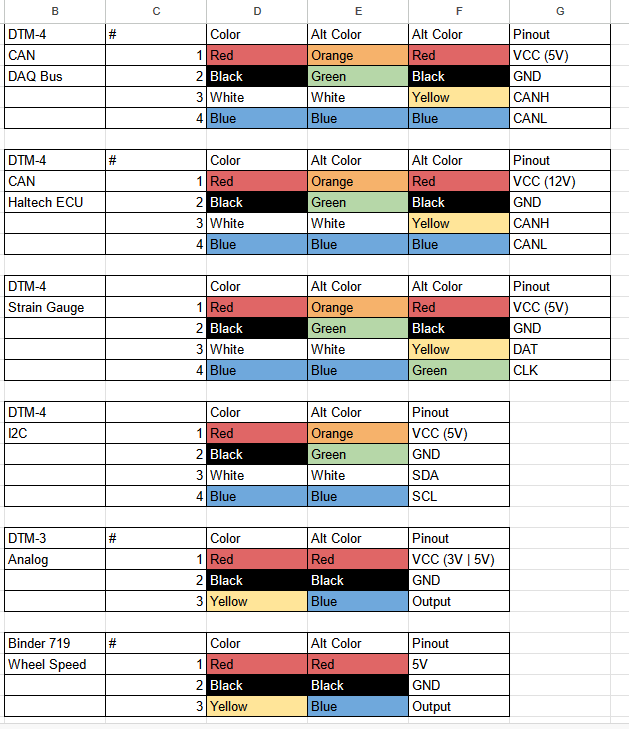
\includegraphics[width=5in]{images/colors.png}
        \caption{Wire Color Conventions}
        \label{fig:asfsfsfsfsfsfsf}
\end{figure}
The wire length spreadsheet showed the assembly status of each cable, and kept track of its length in CAD, how much to cut (CAD length plus $10\%$), and how much was actually cut.
\begin{figure}[H]
        \centering
        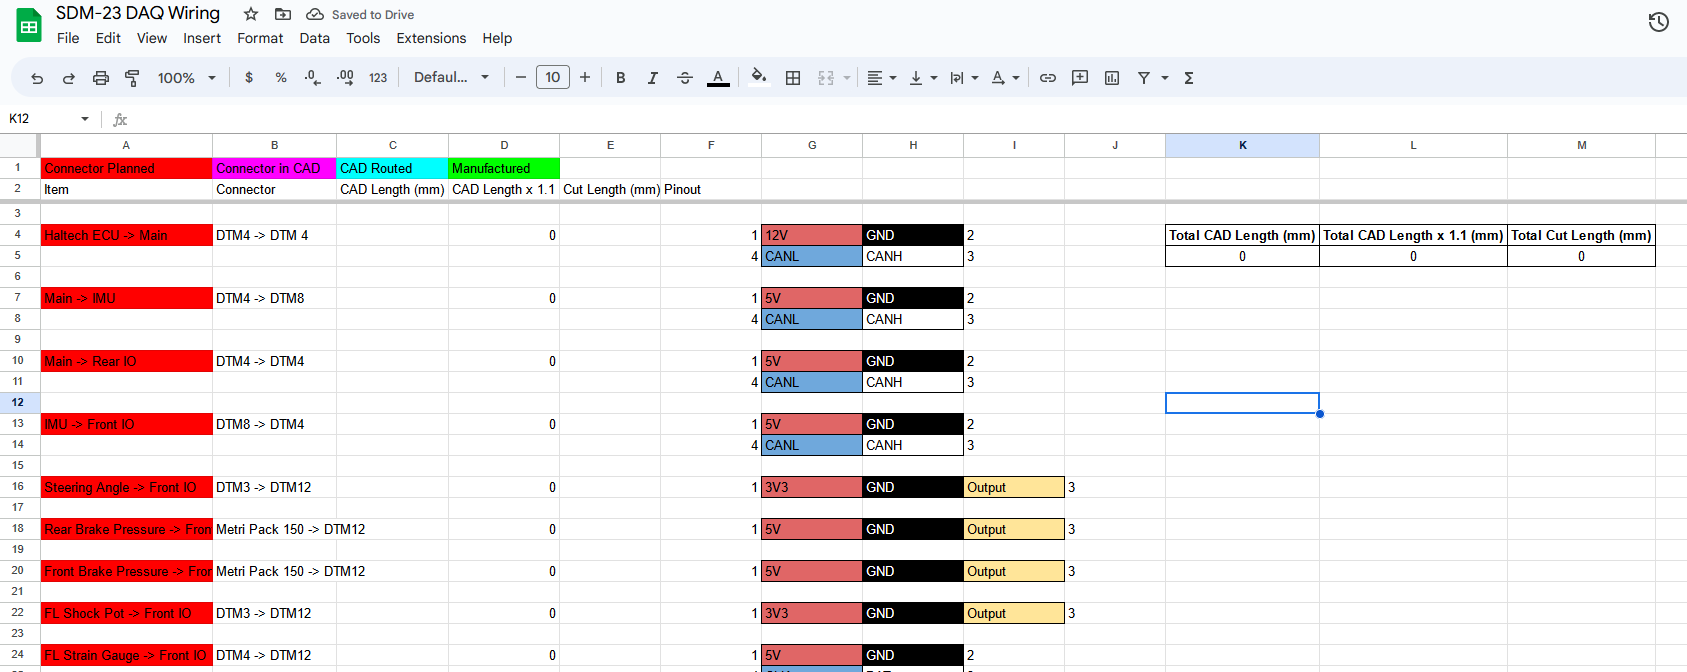
\includegraphics[width=7in]{images/wiring.png}
        \caption{Wire Length Tracking}
        \label{fig:fffsaf}
\end{figure}
The pinout spreadsheet documented what each pin should be connected to.
\begin{figure}[H]
        \centering
        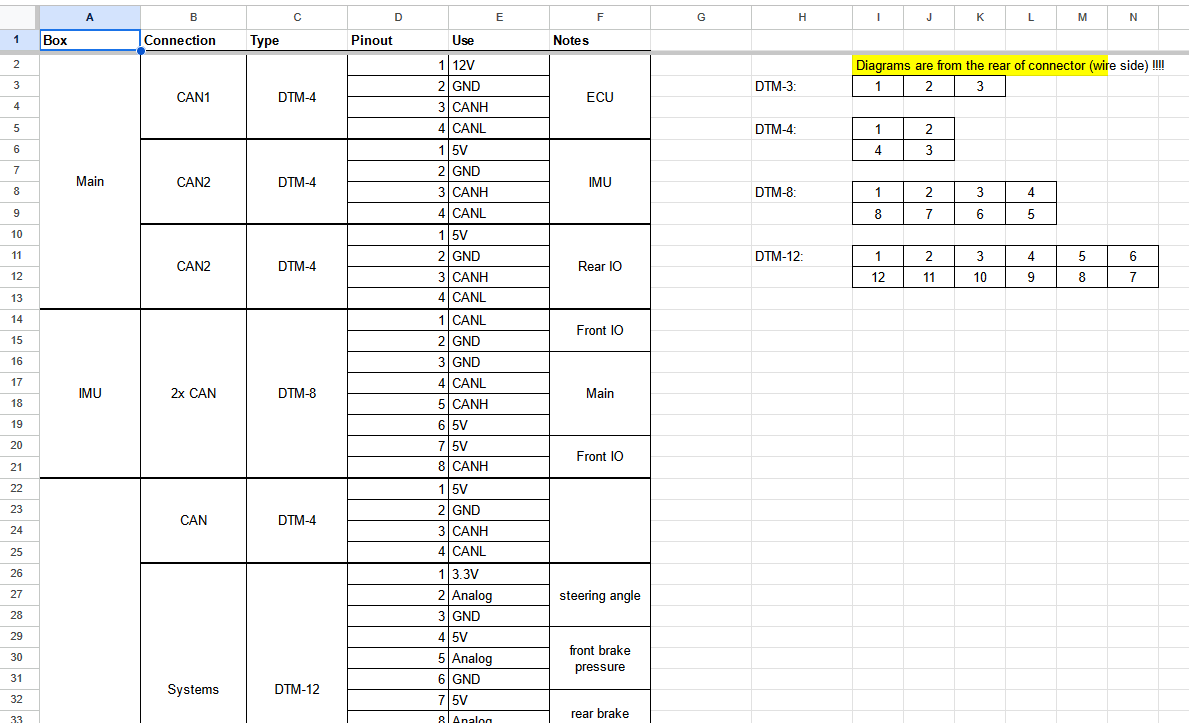
\includegraphics[width=7in]{images/pinouts.png}
        \caption{Box Pinout Documentation}
        \label{fig:hghahhhh}
\end{figure}
These three spreadsheets were instrumental while assembling the connectors and debugging any issues.


\subsection{Strain Gauge Integration}
\subsubsection{Materials and Chemicals Required to Bond the Strain Gauge}
Bonding the MMF403924 Tee Rosette strain gauges required the following:
\begin{itemize}
    \item Personal protective equipment (PPE)
    \item M-Bond 200 Adhesive
    \item M-Bond 200 Catalyst C
    \item M-Prep Conditioner A
    \item M-Prep Neutralizer 5A
\end{itemize}

\subsubsection{Personal protective equipment (PPE)}

Taken directly from the following data sheets: 
\begin{itemize}
    \item M-Bond\textunderscore 200\textunderscore Adhesive\textunderscore SDS\textunderscore V3.0.pdf
    \item M-Bond\textunderscore 200\textunderscore Catalyst\textunderscore C\textunderscore SDS\textunderscore V3.0.pdf
    \item M-Prep\textunderscore Conditioner\textunderscore A\textunderscore SDS\textunderscore V2.pdf
    \item M-Prep\textunderscore Neutralizer\textunderscore 5A\textunderscore SDS\textunderscore V2.pdf
\end{itemize}
\begin{quote} 
``Wear protective eye glasses for protection against liquid splashes. Wear eye protection with side protection. (Recommended: EN166)."
\end{quote}
\begin{quote} 
``Wear impervious gloves. Recommended: Equivalent or similar to EN374.
Gloves should be changed regularly to avoid permeation problems."
\end{quote}
\begin{quote} 
``Body protection:
Wear impervious protective clothing, including boots, lab coat, apron or coveralls,
as appropriate, to prevent skin contact.
Use only in well-ventilated areas. In case of inadequate ventilation wear respiratory protection.
For large quantities - A suitable mask with filter type A may be appropriate.
(Recommended: EN141 or EN405)"
\end{quote}

\subsubsection{M-Bond 200 Adhesive}
Chemical name(s): Ethyl 2-cyanoacrylate
\vspace{1em}

Use case: Adhesives
\begin{figure}[H]
        \centering
        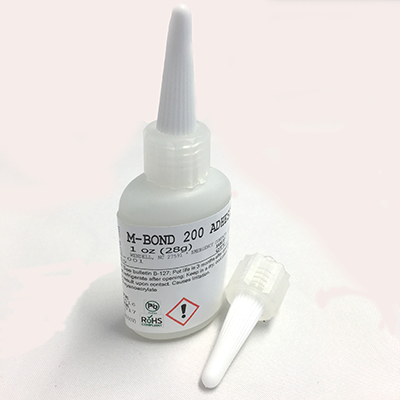
\includegraphics[width=3in]{images/Strain Gauge/M-Bond 200 Adhesive.png}
        \caption{M-Bond 200 Adhesive}
        \label{fig:M-Bond 200 Adhesive}
\end{figure}

\subsubsection{M-Bond 200 Catalyst C}
Chemical name(s): Propan-2-ol and N-Phenyldiethanolamine

\vspace{1em}

Use case: Adhesives
\begin{figure}[H]
        \centering
        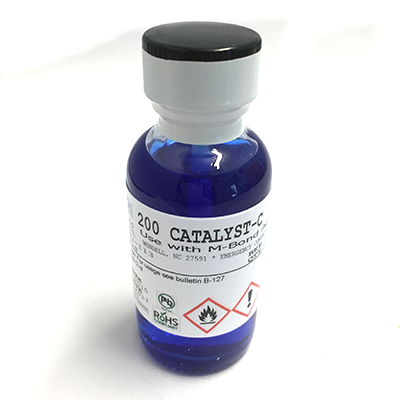
\includegraphics[width=3in]{images/Strain Gauge/M-Bond 200 Catalyst C.png}
        \caption{M-Bond 200 Catalyst C}
        \label{fig:M-Bond 200 Catalyst C}
\end{figure}

\subsubsection{M-Prep Conditioner A}
Chemical name(s): Phosphoric Acid

\vspace{1em}

Use case: PC14 Metal surface treatment products, including galvanic and electroplating products

\begin{figure}[H]
        \centering
        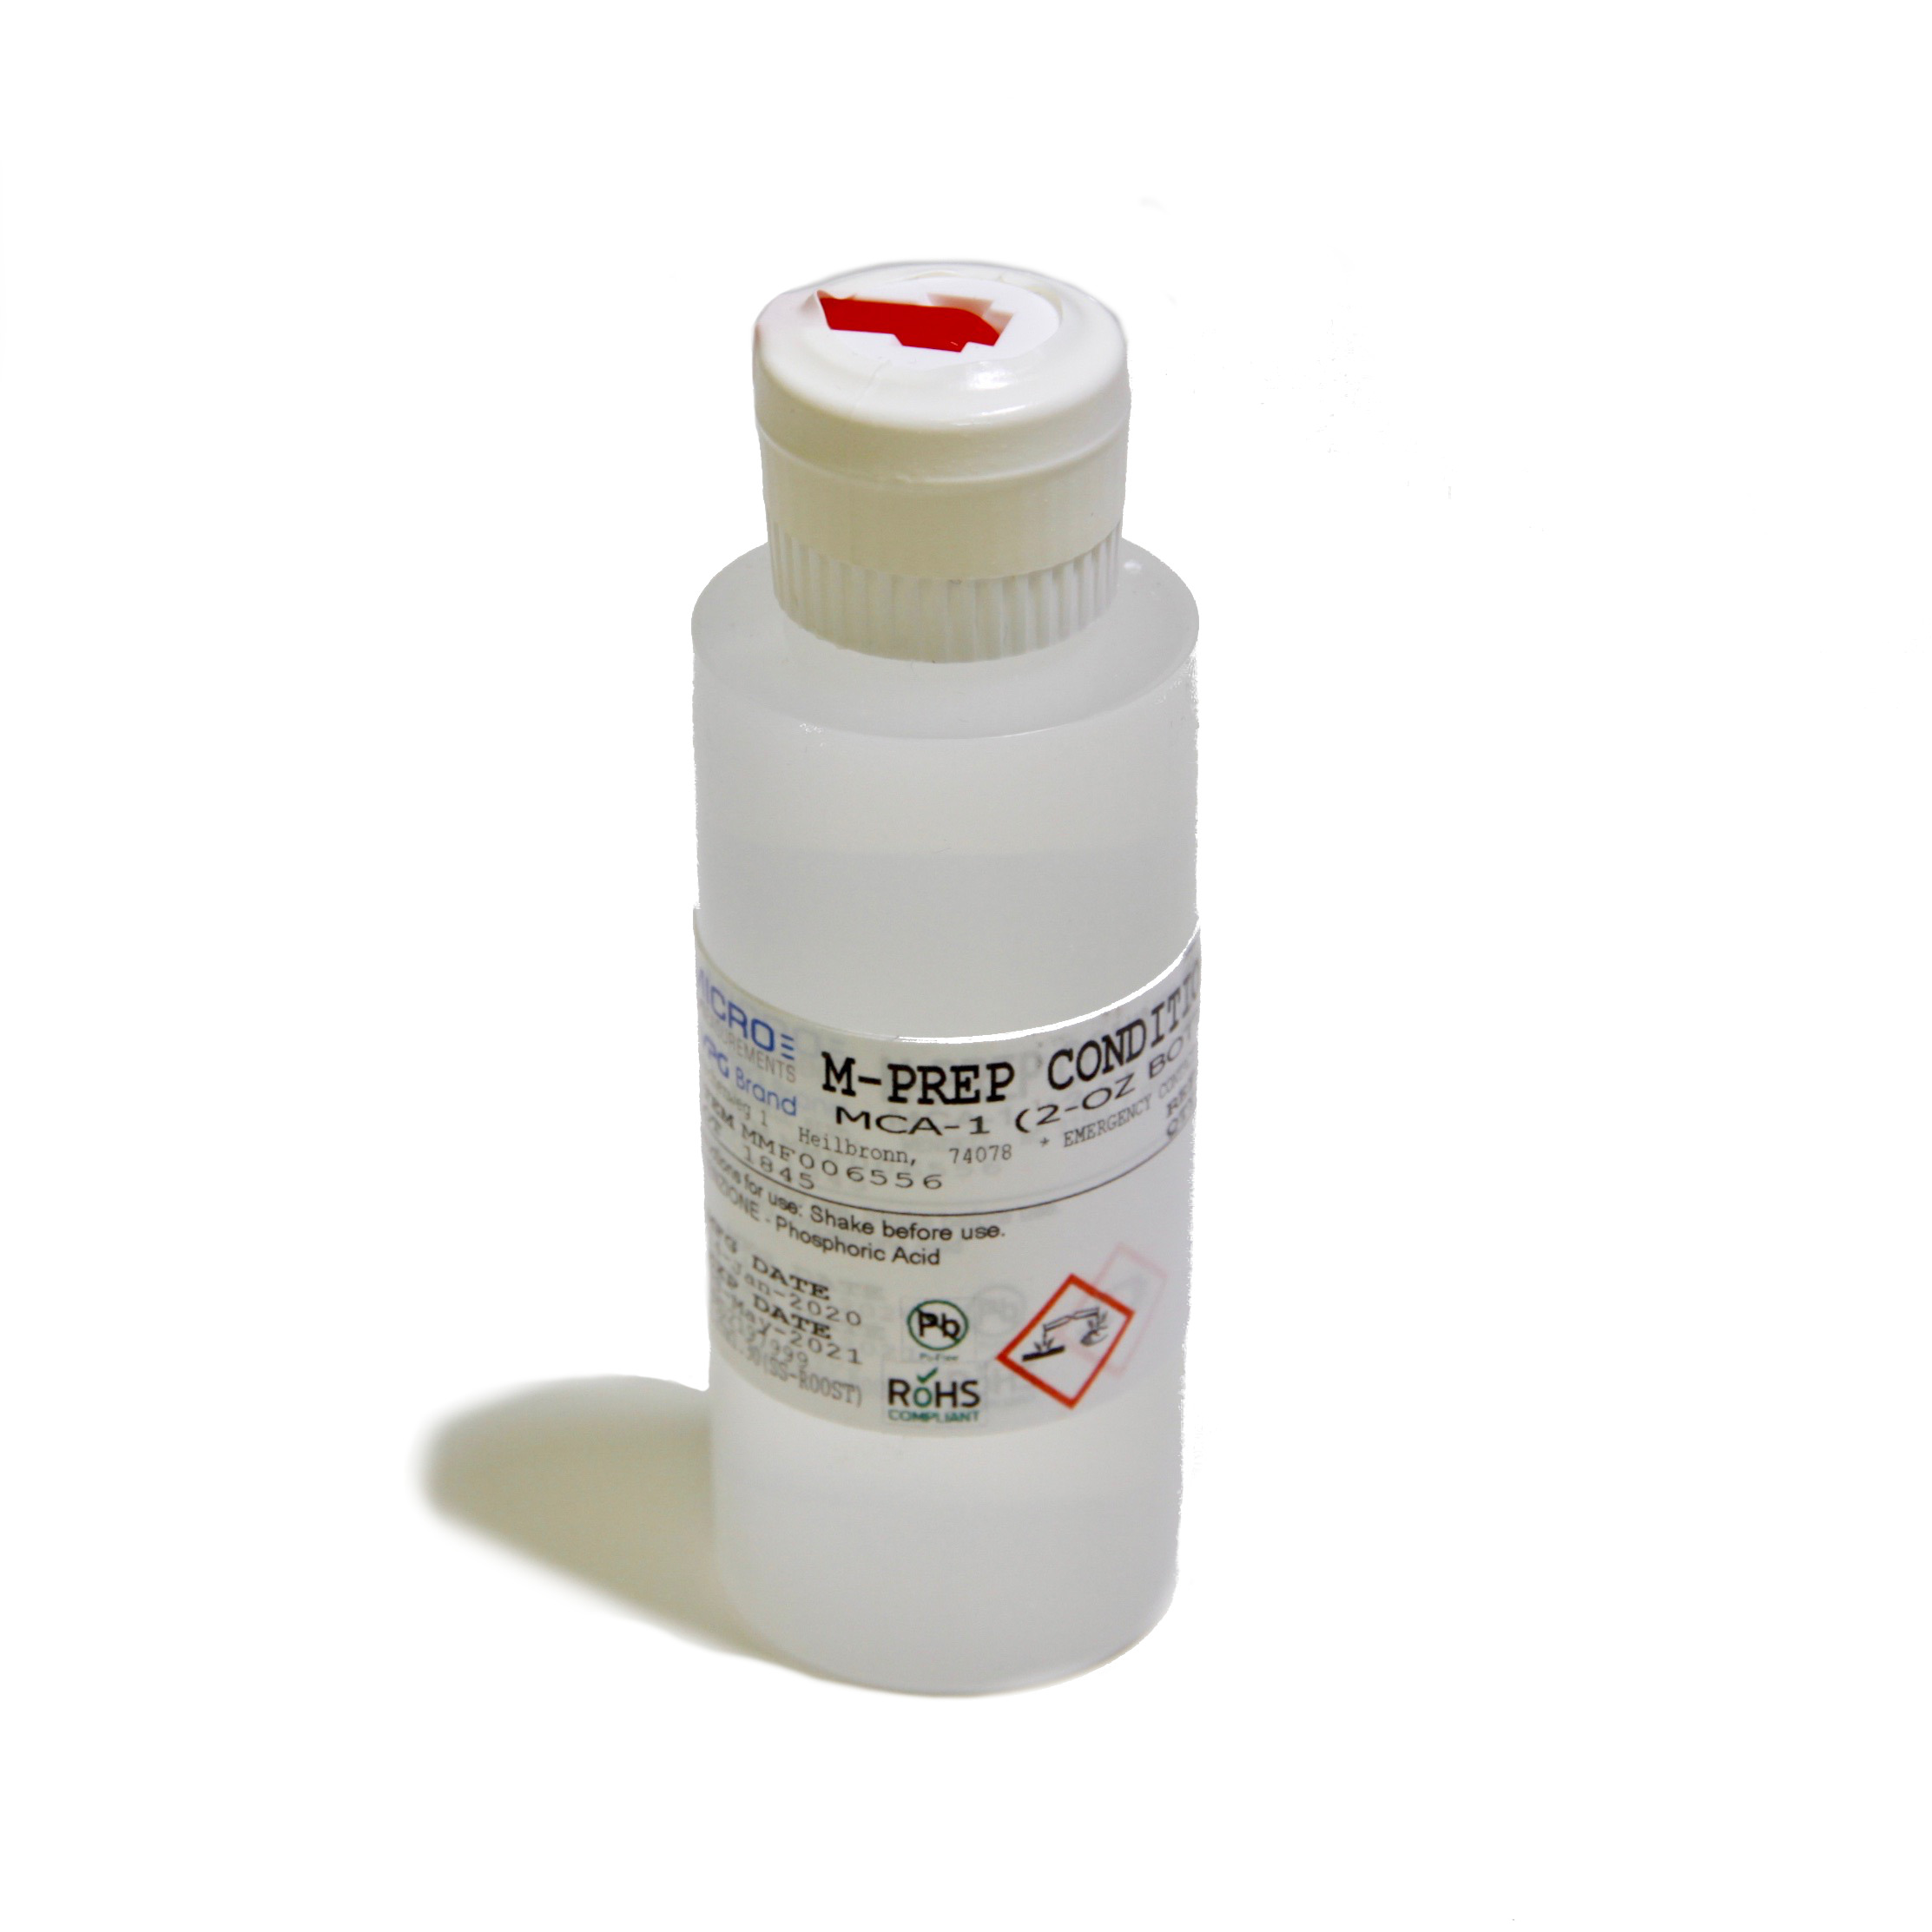
\includegraphics[width=3in]{images/Strain Gauge/M-Prep Conditioner A.jpg}
        \caption{M-Prep Conditioner A}
        \label{fig:M-Prep Conditioner A}
\end{figure}

\subsubsection{M-Prep Neutralizer 5A}
Chemical name(s): Sodium tetraborate pentahydrate 

\vspace{1em}

Use case: PC14 Metal surface treatment products, including galvanic and electroplating products
\begin{figure}[H]
        \centering
        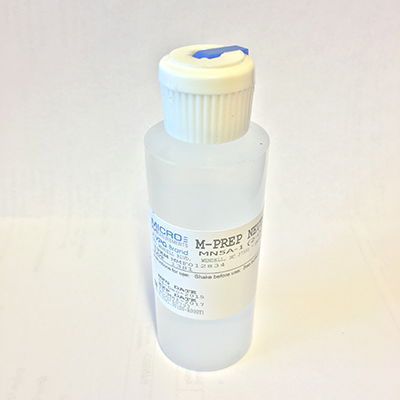
\includegraphics[width=3in]{images/Strain Gauge/M-Prep Neutralizer 5A.png}
        \caption{M-Prep Neutralizer 5A}
        \label{fig:M-Prep Neutralizer 5A}
\end{figure}


\subsubsection{Bonding Process}
According to Instruction Bulletin B-127: Strain Gage Installations with M-Bond 200 Adhesive there are 11 steps needed to bond the gauges. They are as follows.
\vspace{1em}
\begin{enumerate}
    \item Degreasing the bonding suface with CSM Degreaser or GC-6 Isopropyl Alcohol.
    \item "Preliminary dry abrading with 220- or 320-grit silicon-carbide paper is generally required if there is any surface scale or oxide. Final abrading is done by using 320-grit silicon-carbide paper on surfaces thoroughly wetted with M-Prep Conditioner A; this is followed by wiping dry with a gauze sponge. Repeat this wet abrading process with 400-grit silicon-carbide paper, then dry by slowly wiping through with a gauze sponge" (Instruction Bulletin B-127)
    \item Using M-Prep Neutralizer 5A and cotton tip apply to the intended bonding area. Then use a gauze to slowly dry the surface making sure to not wipe back and forth as this could recontaminate the surface.
    \item Using a pair of tweezers extract the Tee Rosette strain gauge from the envelope placing it bonding side down. The tape the gauge. Slowly lift the tape at roughly at a  45 degree angle.
    \item Tape the gauge onto the bonding surface.
    \item Lift the tape at roughly at a 45 degree angle making sure "the specimen approximately 1/2 in [10 mm] beyond the terminal."
    \item The following three steps need to be performed within 3 to 5 seconds.
    \item Apply a sparingly amount of M-Bond 200 catalyst to the strain gauge. 
    \item Apply about one to two drops of the M-Bond 200 adhesive to the corner of the lifted tape area. For curved surfaces like a rod apply a very small amount to avoid the substance from dripping. 
    \item Immediately flip the tape. Then using a gauze wipe the tape in a single stroke.
    \item Apply pressure with your thumb to area that the gauge was bonded to. Hold this pressure for about a minute. The longer the better though as removing your thumb too soon could cause the bond to be very weak. For example, when lifting the tape the gauge could peel off. Note: If the gauges are large or if the surface is curved one should wait two minutes instead of one.
    \item It is not required to remove the tape immediately. In fact unless you are soldering or adding something like a  coating you should leave the tape on. When ready to remove the tape slowly peel it directly over itself. This will prevent the gauge from being damaged or lifted with the tape. 
\end{enumerate}

"FINAL INSTALLATION PROCEDURE":
Solder the gauges. 
Remove any solder flux. 
Apply protective coating.


\subsubsection{Bonded and Soldered Strain Gauges}
\begin{figure}[H]
        \centering
        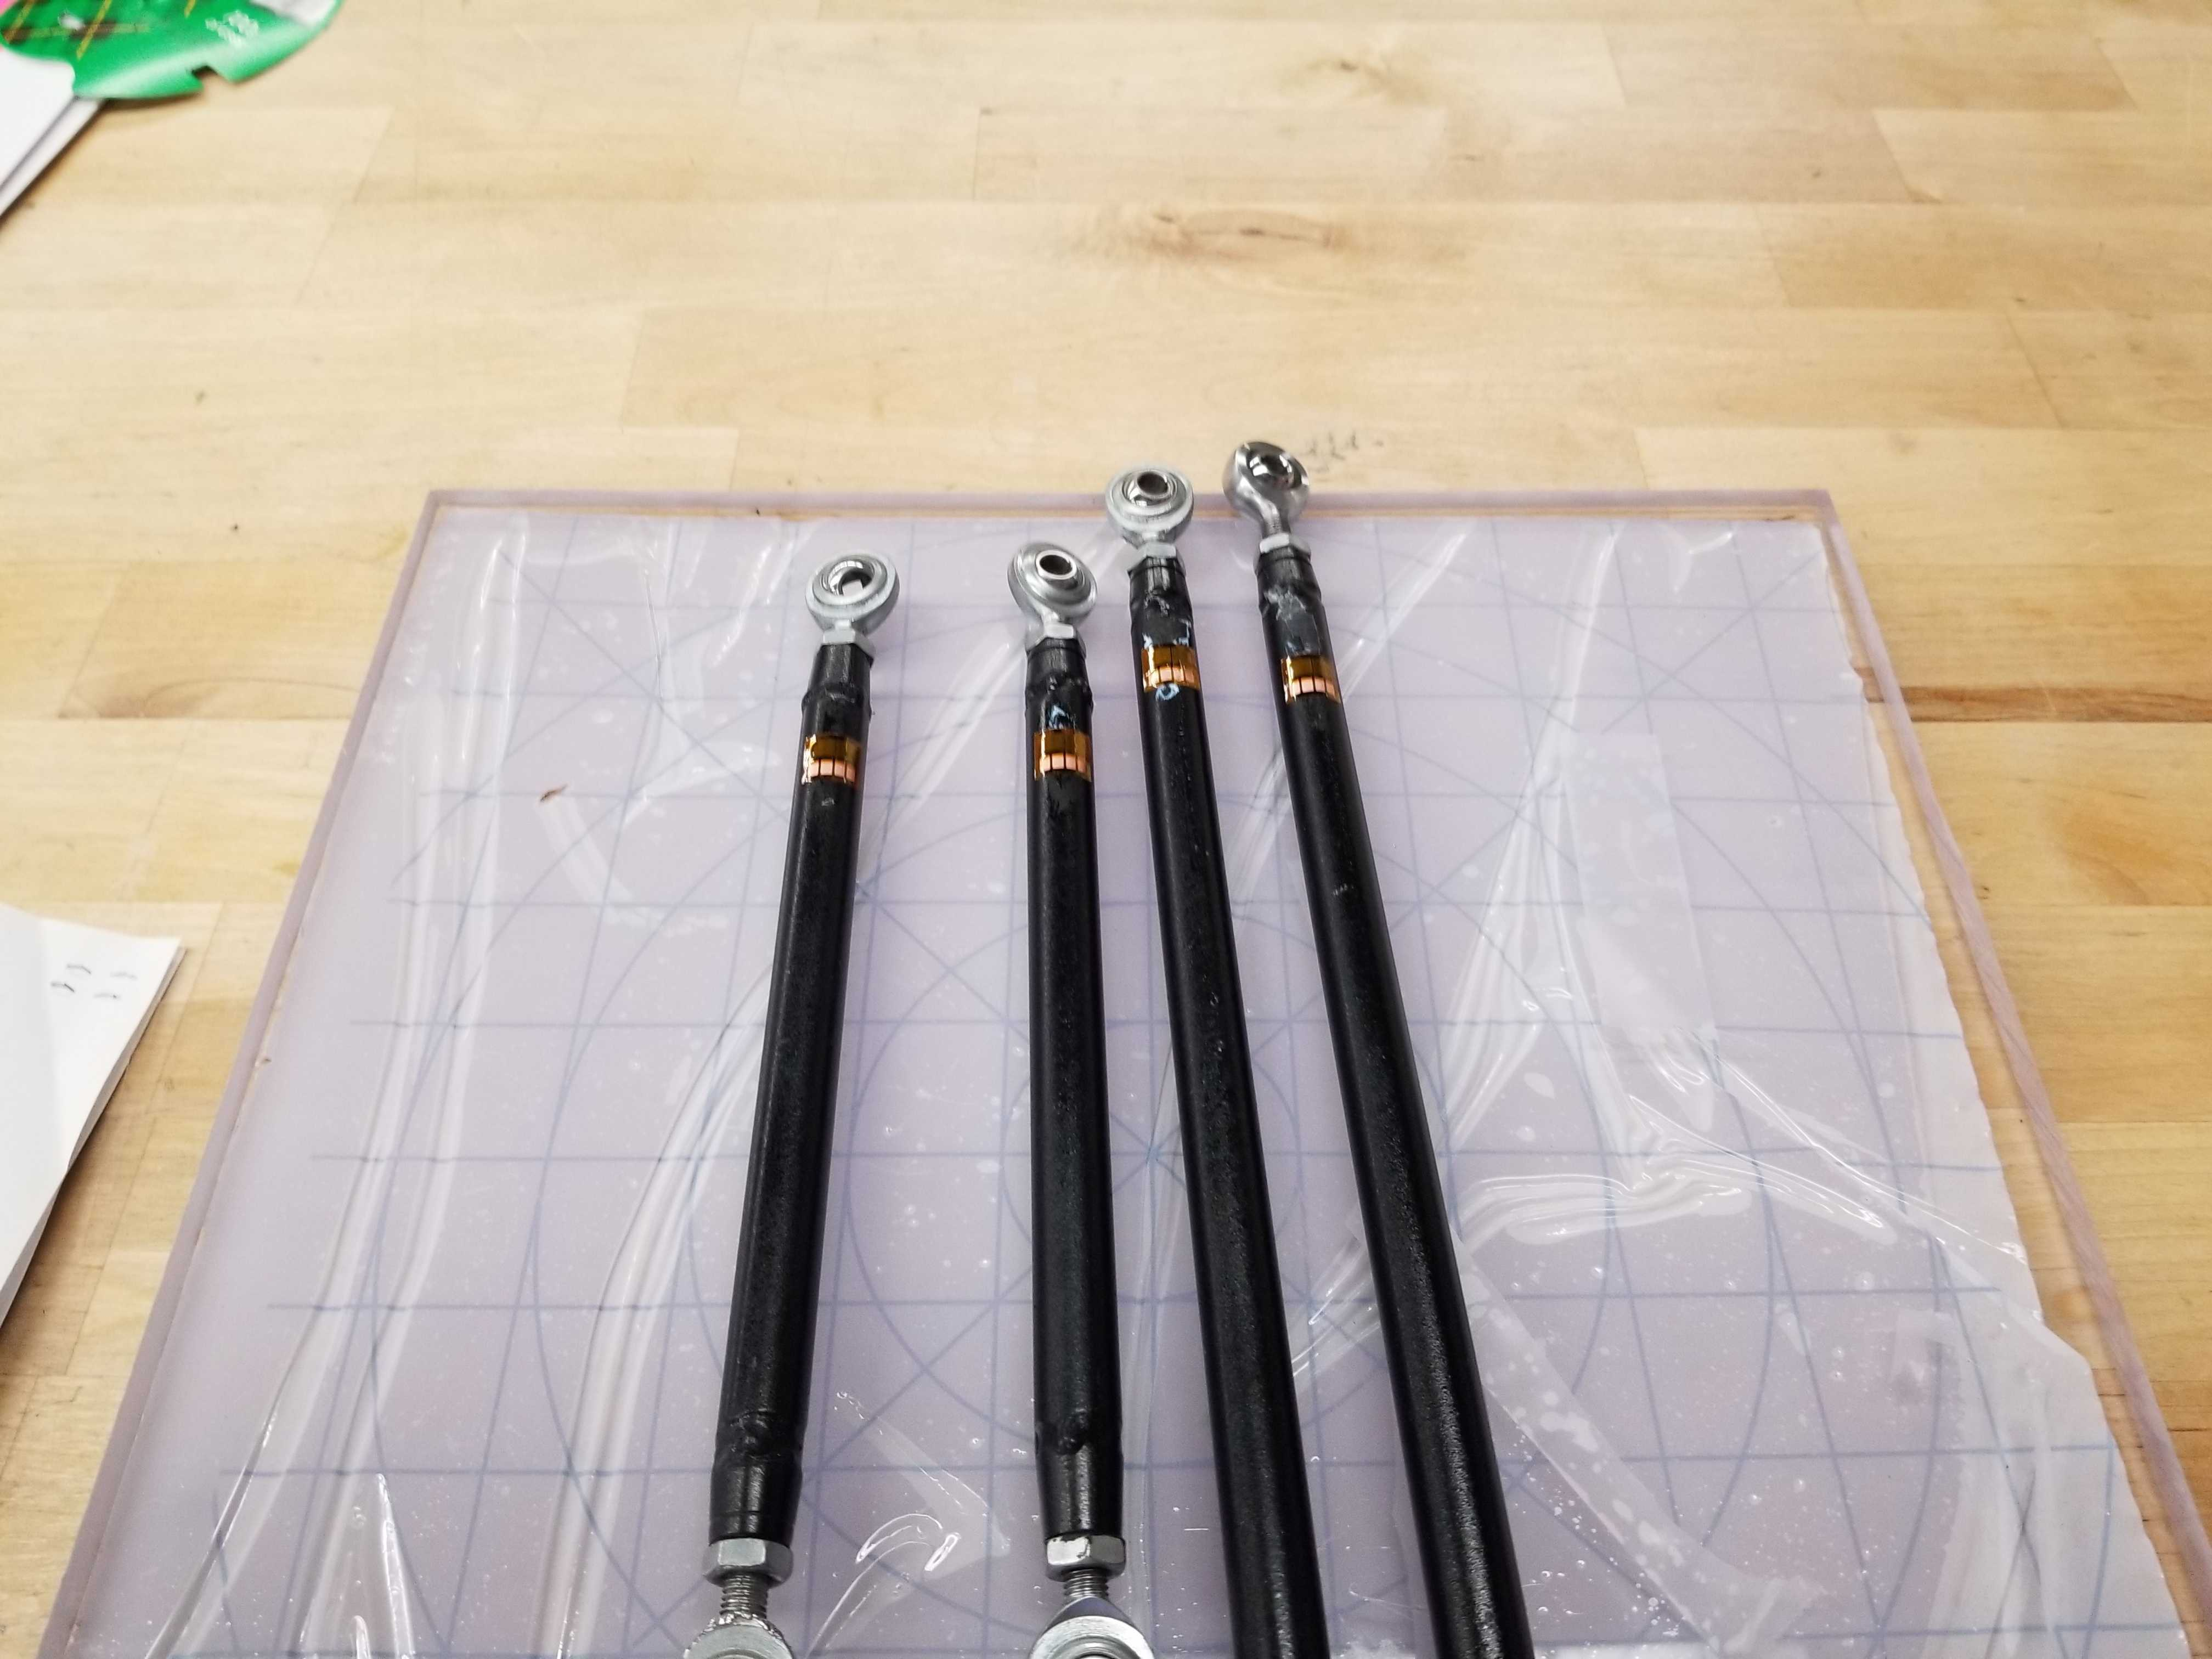
\includegraphics[width=4in]{images/Strain Gauge/straingauge-noleads.jpg}
        \caption{Bonded Strain Gauges}
        \label{fig:straingauge-noleads}
\end{figure}

\begin{figure}[H]
        \centering
        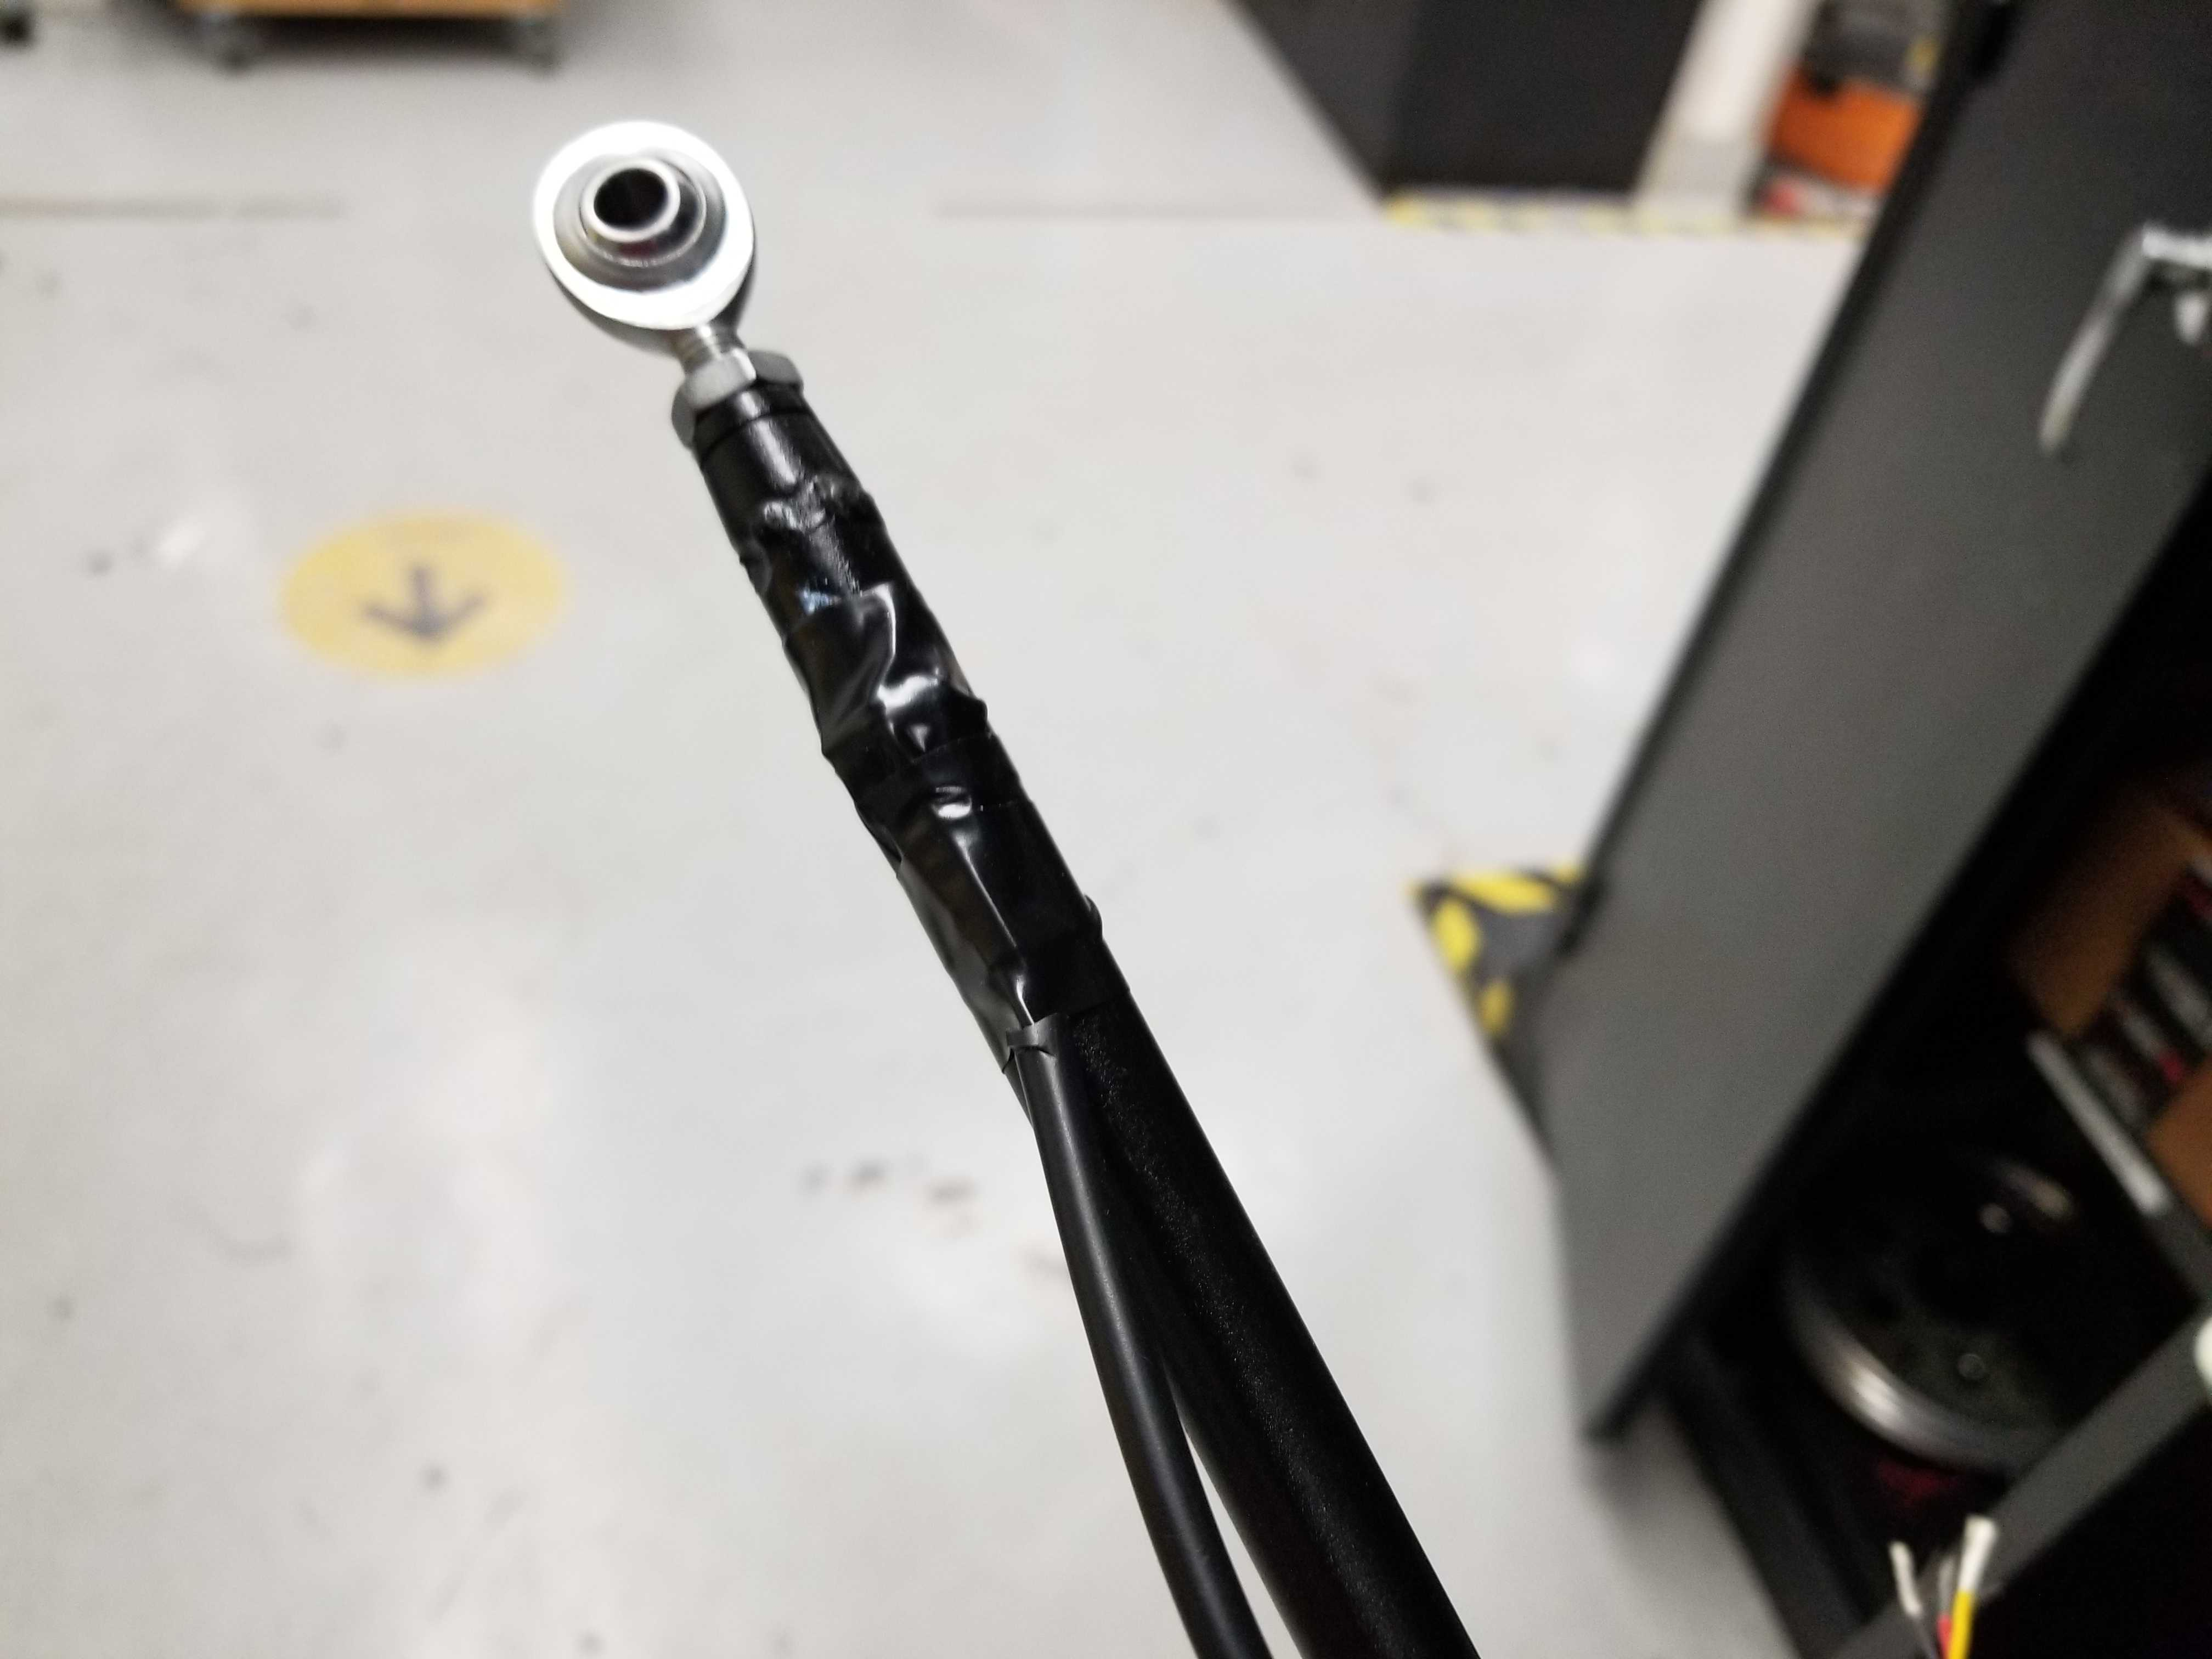
\includegraphics[width=4in]{images/Strain Gauge/straingauge.jpg}
        \caption{Soldered Strain Gauges}
        \label{fig:Soldered Strain Gauges}
\end{figure}


\subsection{Box Assembly}
All 3D-prints were printed by a Creality Ender 3 Pro.
Terminal blocks were screwed in by using electrical tweezers.
The DTM connectors were super glued to their 3D-printed panel mounts.